\documentclass[border=5pt]{standalone}
\usepackage{tikz}
\usetikzlibrary{positioning, patterns, decorations.pathreplacing}
\usetikzlibrary{calc}
\usetikzlibrary{arrows,shapes,backgrounds}

\begin{document}


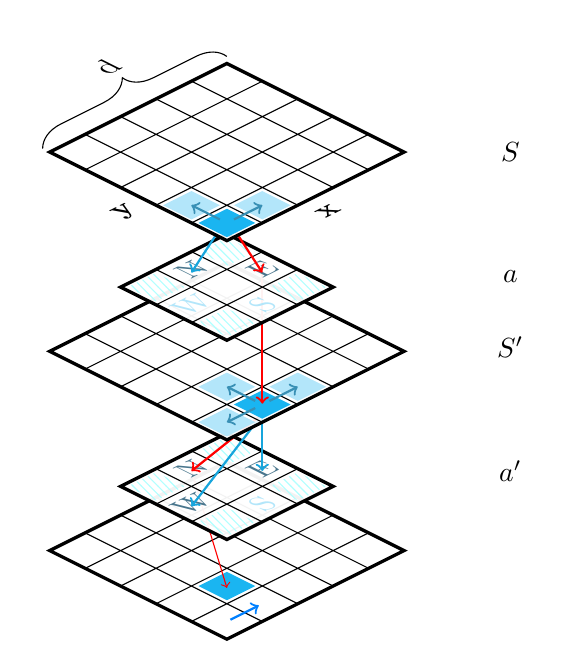
\begin{tikzpicture}[scale=.9,every node/.style={minimum size=1cm},on grid]

\tikzstyle{select arrow}=[->, thick,cyan!70!black]
\tikzstyle{action arrow}=[->, thick,cyan!90!black]
\tikzstyle{action good}=[thick,cyan!50!black]
\tikzstyle{action bad}=[thick,cyan!30]
\tikzstyle{active neuron}=[cyan!90]
\tikzstyle{selected neuron}=[cyan!30]
\tikzstyle{bad action}=[pattern=north west lines, pattern color=cyan!30]

%FINAL STATE. plane at the bottom
\begin{scope}[
            yshift=-160,every node/.append style={
            yslant=0.5,xslant=-1},yslant=0.5,xslant=-1
            ]

        \fill[white,fill opacity=0.9] (0,0) rectangle (2.5,2.5);
        \draw[step=5mm, black] (0,0) grid (2.5,2.5);
        \draw[black,very thick] (0,0) rectangle (2.5,2.5);
        \fill[active neuron] (0.55,0.55) rectangle (0.95,0.95);

\draw[->,thick, blue!50!cyan] (0.3,0.25) -- (0.7,0.25);
\end{scope}

\draw[action arrow, red, thin] (-0.5,-3.25) -- (0,-4.9);

%SECOND ACTION
   \begin{scope}[
    	yshift=-120,every node/.append style={
    	yslant=0.5,xslant=-1},yslant=0.5,xslant=-1
    	             ]
    	\fill[white,fill opacity=.95] (0,0) rectangle (1.5,1.5);
    	\draw[step=5mm, black] (0,0) grid (1.5,1.5);
    	\draw[black,very thick] (0,0) rectangle (1.5,1.5);

\fill[bad action] (0.05,0.05) rectangle (0.45,0.45);
\fill[bad action] (1.05,0.05) rectangle (1.45,0.45);
\fill[bad action] (1.05,1.05) rectangle (1.45,1.45);
\fill[bad action] (0.05,1.05) rectangle (0.45,1.45);

\node[action good] at (0.25,0.75) {W};
\node[action good] at (1.25,0.75) {E};
\node[action good] at (0.75,1.25) {N};
\node[action bad] at (0.75,0.25) {S};
    \end{scope}

\draw[action arrow] (0.5,-2.45) -- (0.5,-3.25);
\draw[action arrow, red] (0.5,-2.45) -- (-0.5,-3.25);
\draw[action arrow] (0.5,-2.45) -- (-0.5,-3.75);

%SECOND STATE
\begin{scope}[
            yshift=-80,every node/.append style={
            yslant=0.5,xslant=-1},yslant=0.5,xslant=-1
            ]

        \fill[white,fill opacity=0.9] (0,0) rectangle (2.5,2.5);
        \draw[step=5mm, black] (0,0) grid (2.5,2.5);
        \draw[black,very thick] (0,0) rectangle (2.5,2.5);
        \fill[active neuron] (0.55,0.05) rectangle (0.95,0.45);  
		\fill[selected neuron] (0.05,0.05) rectangle (0.45,0.45);
		\fill[selected neuron] (1.05,0.05) rectangle (1.45,0.45);
		\fill[selected neuron] (0.55,0.55) rectangle (0.95,0.95);

\draw[select arrow] (0.85,0.25) -- (1.25,0.25);
\draw[select arrow] (0.75,0.35) -- (0.75,.75);
\draw[select arrow] (0.65,0.25) -- (0.25,0.25);
\end{scope}

\draw[action arrow, red] (0.5,-0.45) -- (0.5,-2.3);

%FIRST ACTION
   \begin{scope}[
    	yshift=-40,every node/.append style={
    	yslant=0.5,xslant=-1},yslant=0.5,xslant=-1
    	             ]
    	\fill[white,fill opacity=.95] (0,0) rectangle (1.5,1.5);
    	\draw[step=5mm, black] (0,0) grid (1.5,1.5);
    	\draw[black,very thick] (0,0) rectangle (1.5,1.5);

\fill[bad action] (0.05,0.05) rectangle (0.45,0.45);
\fill[bad action] (1.05,0.05) rectangle (1.45,0.45);
\fill[bad action] (1.05,1.05) rectangle (1.45,1.45);
\fill[bad action] (0.05,1.05) rectangle (0.45,1.45);

\node[action bad] at (0.25,0.75) {W};
\node[action good] at (1.25,0.75) {E};
\node[action good] at (0.75,1.25) {N};
\node[action bad] at (0.75,0.25) {S};
    \end{scope}

\draw[action arrow, red] (0.125,0.125) -- (0.5,-0.45);
\draw[action arrow] (-0.125,0.125) -- (-0.5,-0.45);

%INITIAL STATE. plane at the top
\begin{scope}[
            every node/.append style={
            yslant=0.5,xslant=-1},yslant=0.5,xslant=-1
            ]

        \fill[white,fill opacity=0.9] (0,0) rectangle (2.5,2.5);
        \draw[step=5mm, black] (0,0) grid (2.5,2.5);
        \draw[black,very thick] (0,0) rectangle (2.5,2.5);
        \fill[active neuron] (0.05,0.05) rectangle (0.45,0.45);
		\fill[selected neuron] (0.55,0.05) rectangle (0.95,0.45);
		\fill[selected neuron] (0.05,0.55) rectangle (0.45,0.95);

\draw [decorate,decoration={brace,amplitude=10pt}] (0,2.6) -- (2.6,2.6);
\node at (1.6,3.3) {d};

\draw[select arrow] (0.25,0.35) -- (0.25,0.75);
\draw[select arrow] (0.35,0.25) -- (0.75,0.25);

\node at (1.125,-0.3) {\textbf{x}};
\node at (-0.3,1.125) {\textbf{y}};

\end{scope}

\node at (4,1.25) {$S$};
\node at (4,-0.5) {$a$};
\node at (4,-1.5) {$S'$};
\node at (4,-3.25) {$a'$};

\end{tikzpicture}
\end{document}